% LaTeX Article Template - customizing header and footer
\documentclass{article}

\newtheorem{thm}{Theorem}

% Set left margin - The default is 1 inch, so the following
% command sets a 1.25-inch left margin.
\setlength{\oddsidemargin}{0.25in}

% Set width of the text - What is left will be the right margin.
% In this case, right margin is 8.5in - 1.25in - 6in = 1.25in.
\setlength{\textwidth}{6in}

% Set top margin - The default is 1 inch, so the following
% command sets a 0.75-inch top margin.
\setlength{\topmargin}{-0.25in}

% Set height of the header
\setlength{\headheight}{0.3in}

% Set vertical distance between the header and the text
\setlength{\headsep}{0.2in}

% Set height of the text
\setlength{\textheight}{9in}

% Set vertical distance between the text and the
% bottom of footer
\setlength{\footskip}{0.1in}

% Set the beginning of a LaTeX document
\usepackage{multirow}
\usepackage{fullpage}
\usepackage{graphicx}
\usepackage{amsthm}
\usepackage{amssymb}
\usepackage{amssymb}
\usepackage{algpseudocode}
\graphicspath{%
    {converted_graphics/}% inserted by PCTeX
    {/}% inserted by PCTeX
}
%%%%%%%%%%%%%%%%%%%%%%%%%%%%%




\begin{document}\title{Homework $0$\\ Computer Science \\ Spring 2017\\ B351}         % Enter your title between curly braces
\author{Steven Myers}        % Enter your name between curly braces
\date{\today}          % Enter your date or \today between curly braces
\maketitle


% Redefine "plain" pagestyle
\makeatother     % `@' is restored as a "non-letter" character




% Set to use the "plain" pagestyle
\pagestyle{plain}
All the work herein is mine.

\section*{Answers}

\begin{enumerate}
\item $f(x) = x^2$ \begin{verbatim}$f(x) = x^2$\end{verbatim}
\item $g(x,y) = \frac{x - 1}{y + 2}$
\end{enumerate}
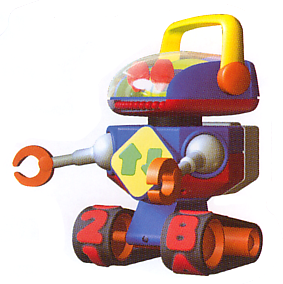
\includegraphics[scale=0.5]{robot}

To bold, \begin{verbatim} \textbf{robot} \end{verbatim} \textbf{robot}
To Italicize, \begin{verbatim} \textit{robot} \end{verbatim} \textit{robot}

\end{document}
